
\section{test}

	\begin{figure} [b]
	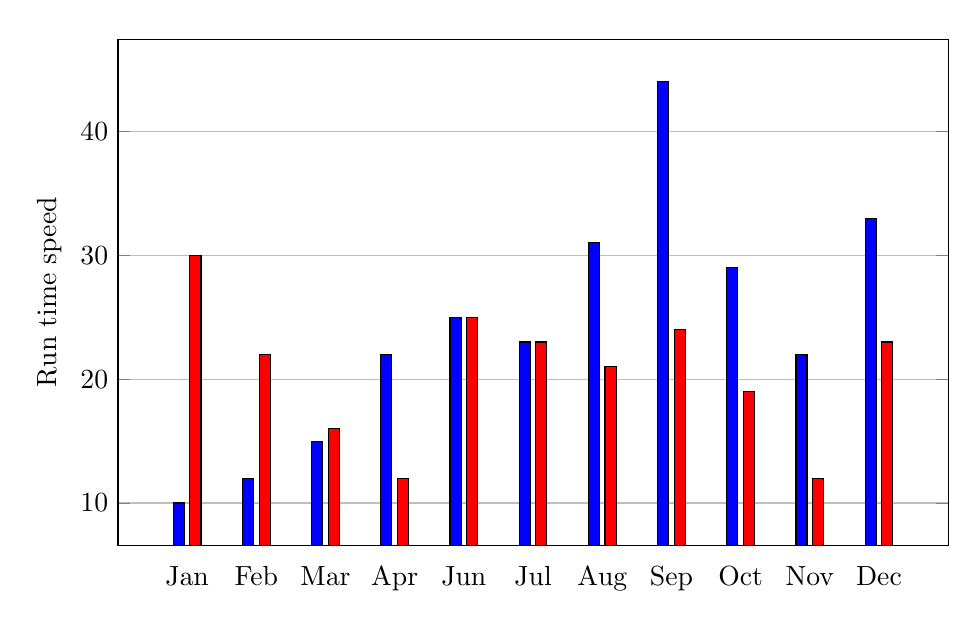
\begin{tikzpicture}	
	\begin{axis} [
	width=1.0\linewidth,      height = 8cm, 
     major x tick style = transparent,
      xtick = data,
	ybar,
	bar width=4pt,
	ymajorgrids = true,
    ylabel = {Run time speed},
       scaled y ticks = false,
    symbolic x coords={Jan, Feb, Mar, Apr, Jun, Jul, Aug, Sep, Oct, Nov, Dec},
	]
	\addplot[ybar,fill=blue] coordinates { (Jan, 10) (Feb, 12) (Mar,15) (Apr,22) (Jun,25) (Jul,23) (Aug,31) (Sep,44) (Oct,29) (Nov,22) (Dec,33) };
	\addplot[ybar,fill=red] coordinates { (Jan, 30) (Feb, 22) (Mar,16) (Apr,12) (Jun,25) (Jul,23) (Aug,21) (Sep,24) (Oct,19) (Nov,12) (Dec,23) };
	\end{axis}
	\end{tikzpicture}
	\caption{Chart name.}
	\label{fig:annu}
	\end{figure}
	figure \ref{fig:annu}.
	
	
	\begin{figure} 
 \begin{tikzpicture}
	\begin{axis} [
		width=1\linewidth,   height = 8cm, 
	major x tick style = transparent,
	    xtick = data,
	%grid=major, 
	%zeichnet Koordinatengitter
    symbolic x coords={Jan, Feb, Mar, Apr, May, Jun, Jul, Aug, Sep, Oct, Nov, Dec},
%	xlabel= Kraft $\lbrack{}$ \si{F} $\rbrack$, 
%	xmin=0,
%	xmax=15,
	ylabel= Strom $\lbrack{}$ \si{kA} $\rbrack$,
	ymin=0,
	ystep=0.5,
	ymax=2.0,
	scaled y ticks = false,
	%nodes near coords, % data 값 표시
	% % % % % Ausrichten der Punktbeschriftung
	every node near coord/.append style={font=\scriptsize,/pgf/number format/precision=3}]
	[legend pos=north east]
	\addplot table [x=Month, y=2003] {momGAC.csv}; \addlegendentry{2003}
	\addplot table [x=Month, y=2004] {momGAC.csv}; \addlegendentry{2004}
	\addplot table [x=Month, y=2005] {momGAC.csv}; \addlegendentry{2005}
	\addplot table [x=Month, y=2006] {momGAC.csv}; \addlegendentry{2006}

%   \fill[gray,fill opacity=0.25] (axis cs:5,0) rectangle (axis cs:7,12); %Bereich einfügen

	\end{axis}
	\end{tikzpicture}

		\caption{Chart name.}
		\label{fig:annu}
	\end{figure}
	figure \ref{fig:annu}.
	

	